\chapter {آشنایی با موتور بازی}

\section{ساخت پروژه}

برای اینکه بتوان از موتور بازی‌سازی آنریل استفاده کرد ، ابتدا باید پروژه ای متناسب با کاری که می‌خواهیم انجام دهیم، بسازیم.
\\
برای ساختن پروژه به صورت زیر عمل می‌کنیم.
\\
ابتدا مرورگر آنریل انجین را باز می‌کنیم.


سپس با انتخاب دسته بندی مناسب و انتخاب گزینه‌ی بعدی به صفحه‌ی زیر هدایت می‌شویم. در اینجا  زیرمجموعه‌ی بازی را انتخاب شده است.

\begin{figure}[H]
	\centerline{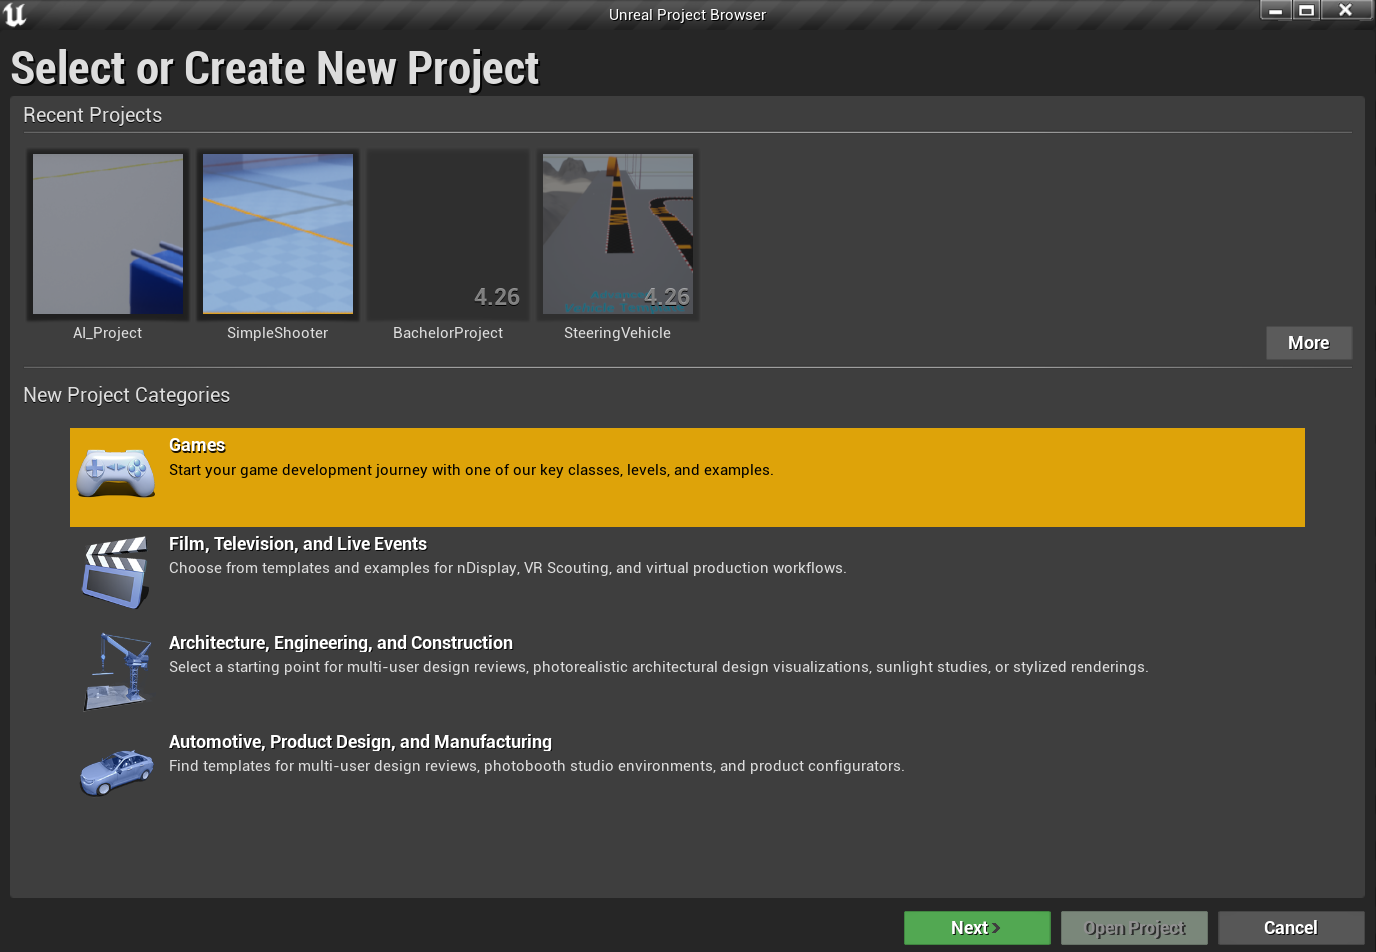
\includegraphics[width=\textwidth,height=\textheight,keepaspectratio]{Figures/Ch2/UnrealEngineBrowser.png}}
	\caption{مرورگر پروژه‌های آنریل}
	\label{fig:Unreal engine Browser}
\end{figure}

\par\bigskip 
\noindent


در اینجا قالب مناسب را انتخاب کرده و گزینه‌ی بعدی را کلیک می‌کنیم.

\begin{figure}[H]
	%\centerline{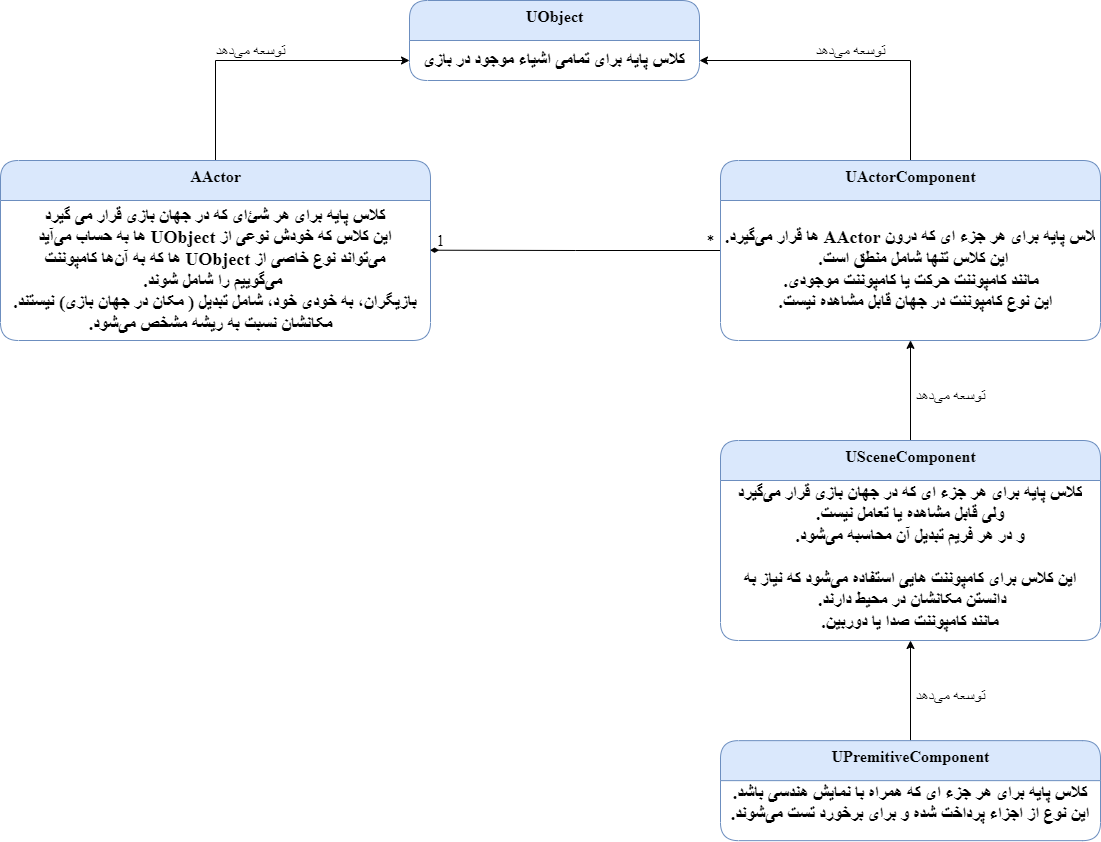
\includegraphics[scale=0.5]{Figures/Ch2/UnrealEngineBasicClassesUML.png}}
	\centerline{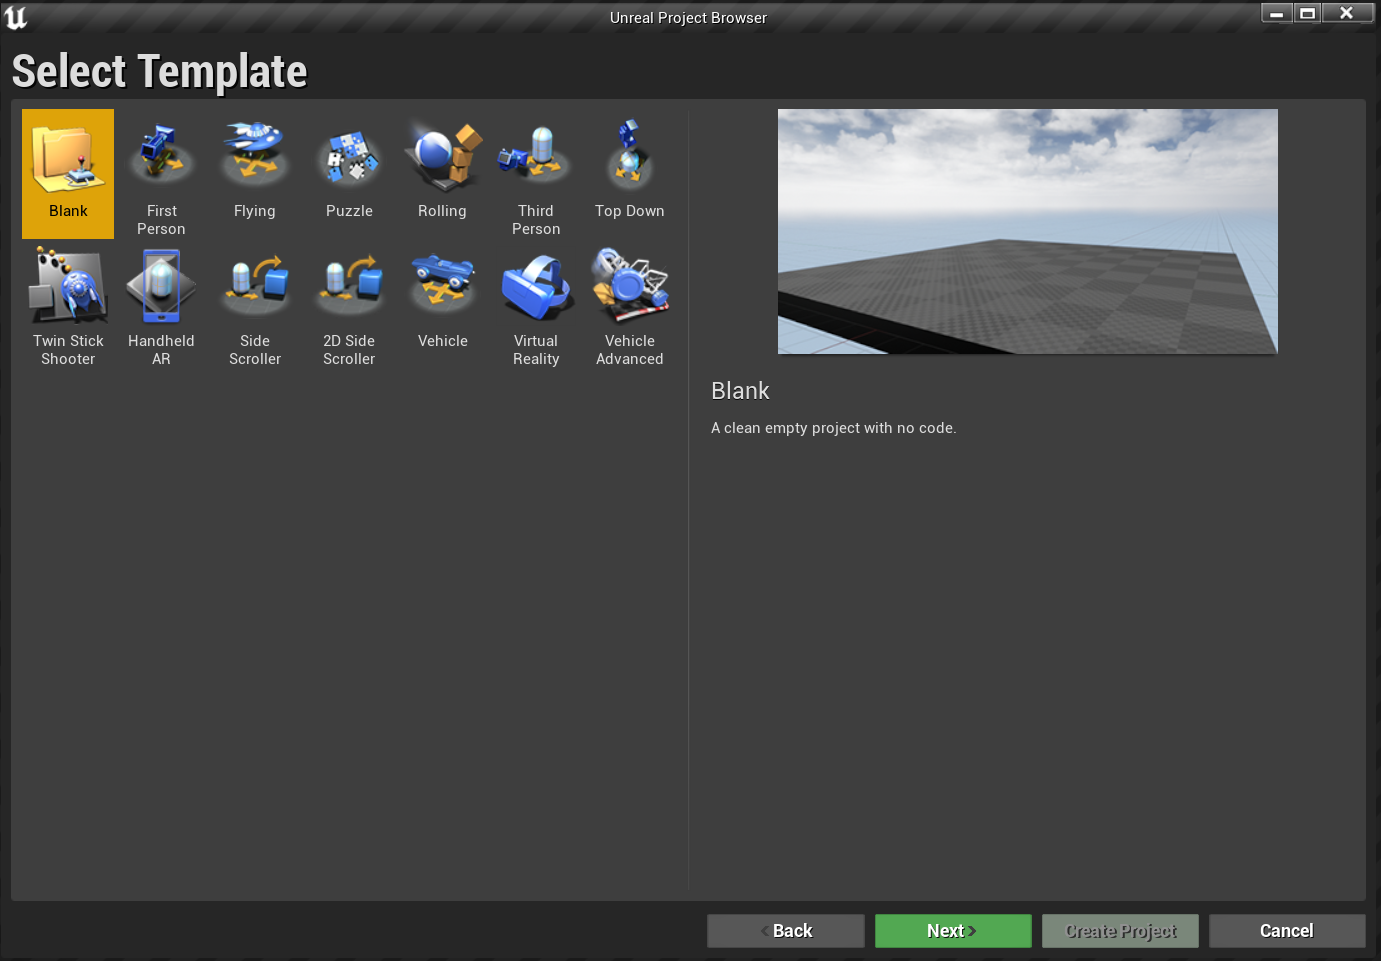
\includegraphics[width=\textwidth,height=\textheight,keepaspectratio]{Figures/Ch2/TemplateSelection.png}}

	\caption{قالب پروژه‌های آنریل}
	\label{fig:Unreal engine Template}
  \end{figure}





در اینجا پس از انجام تنظیمات اولیه پروژه گزینه‌ی ایجاد پروژه را کلیک کرده و پروژه ساخته می‌شود.


\begin{figure}[H]
	\centerline{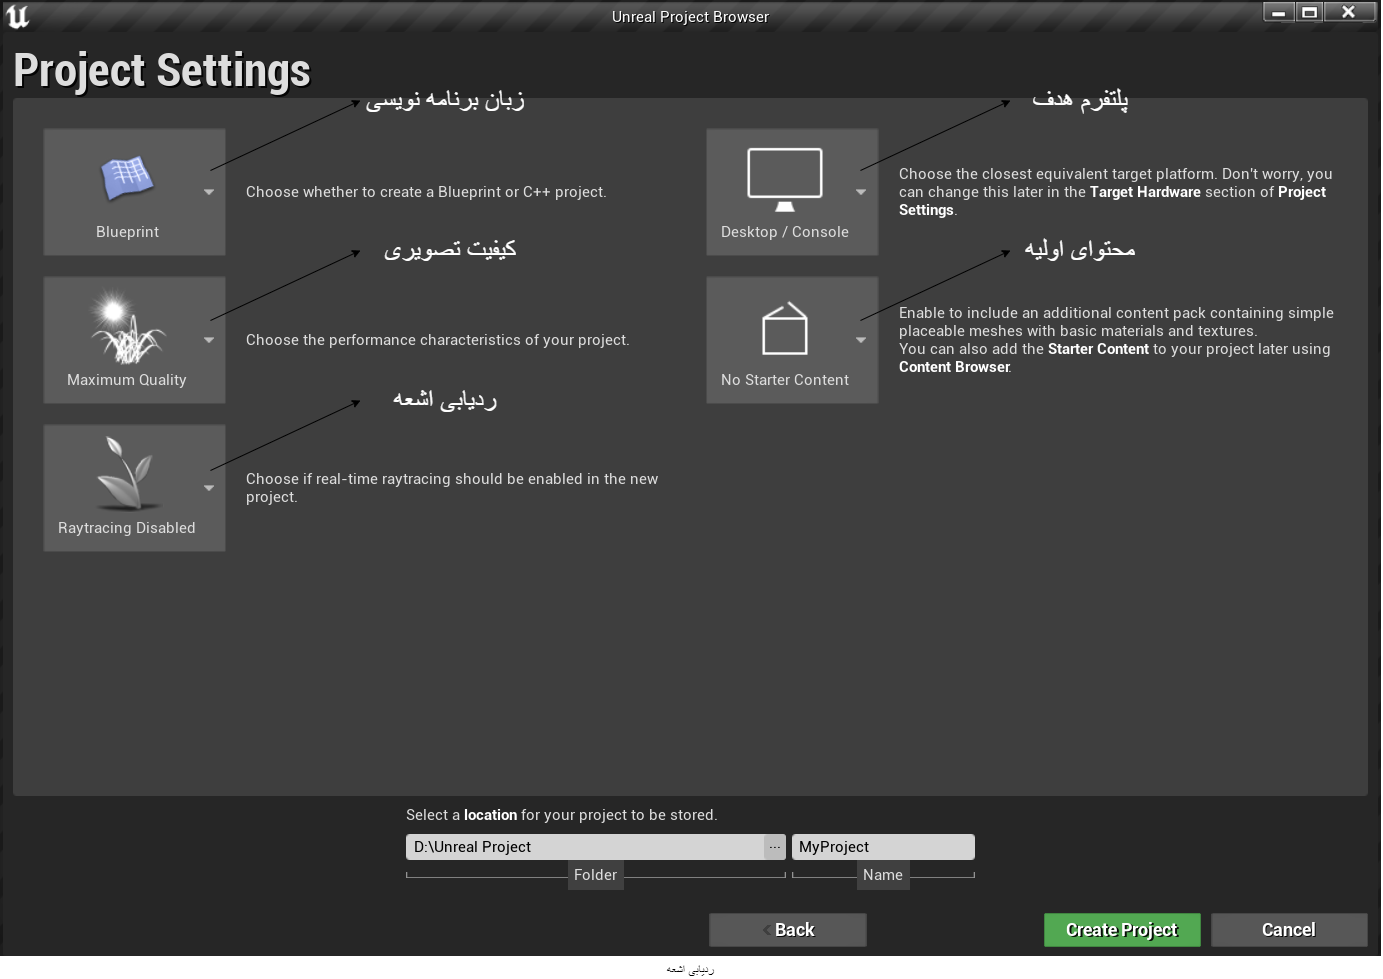
\includegraphics[width=\textwidth,height=\textheight,keepaspectratio]{Figures/Ch2/UnrealEngineProjectSetting.png}}
	\caption{تنظیم پروژه‌های آنریل}
	\label{fig:Unreal engine Setting}
\end{figure}


\section{ویرایشگر آنریل}
زمانی که پروژه ساخته می‌‌شود، ویرایشگر آنریل باز می‌شود. این ویرایشگر شامل پنل های مختلفی است که در عکس شماره زده شده و هر شماره نیز در جدول زیر توضیح داده شده است.

\begin{figure}[H]
	\centerline{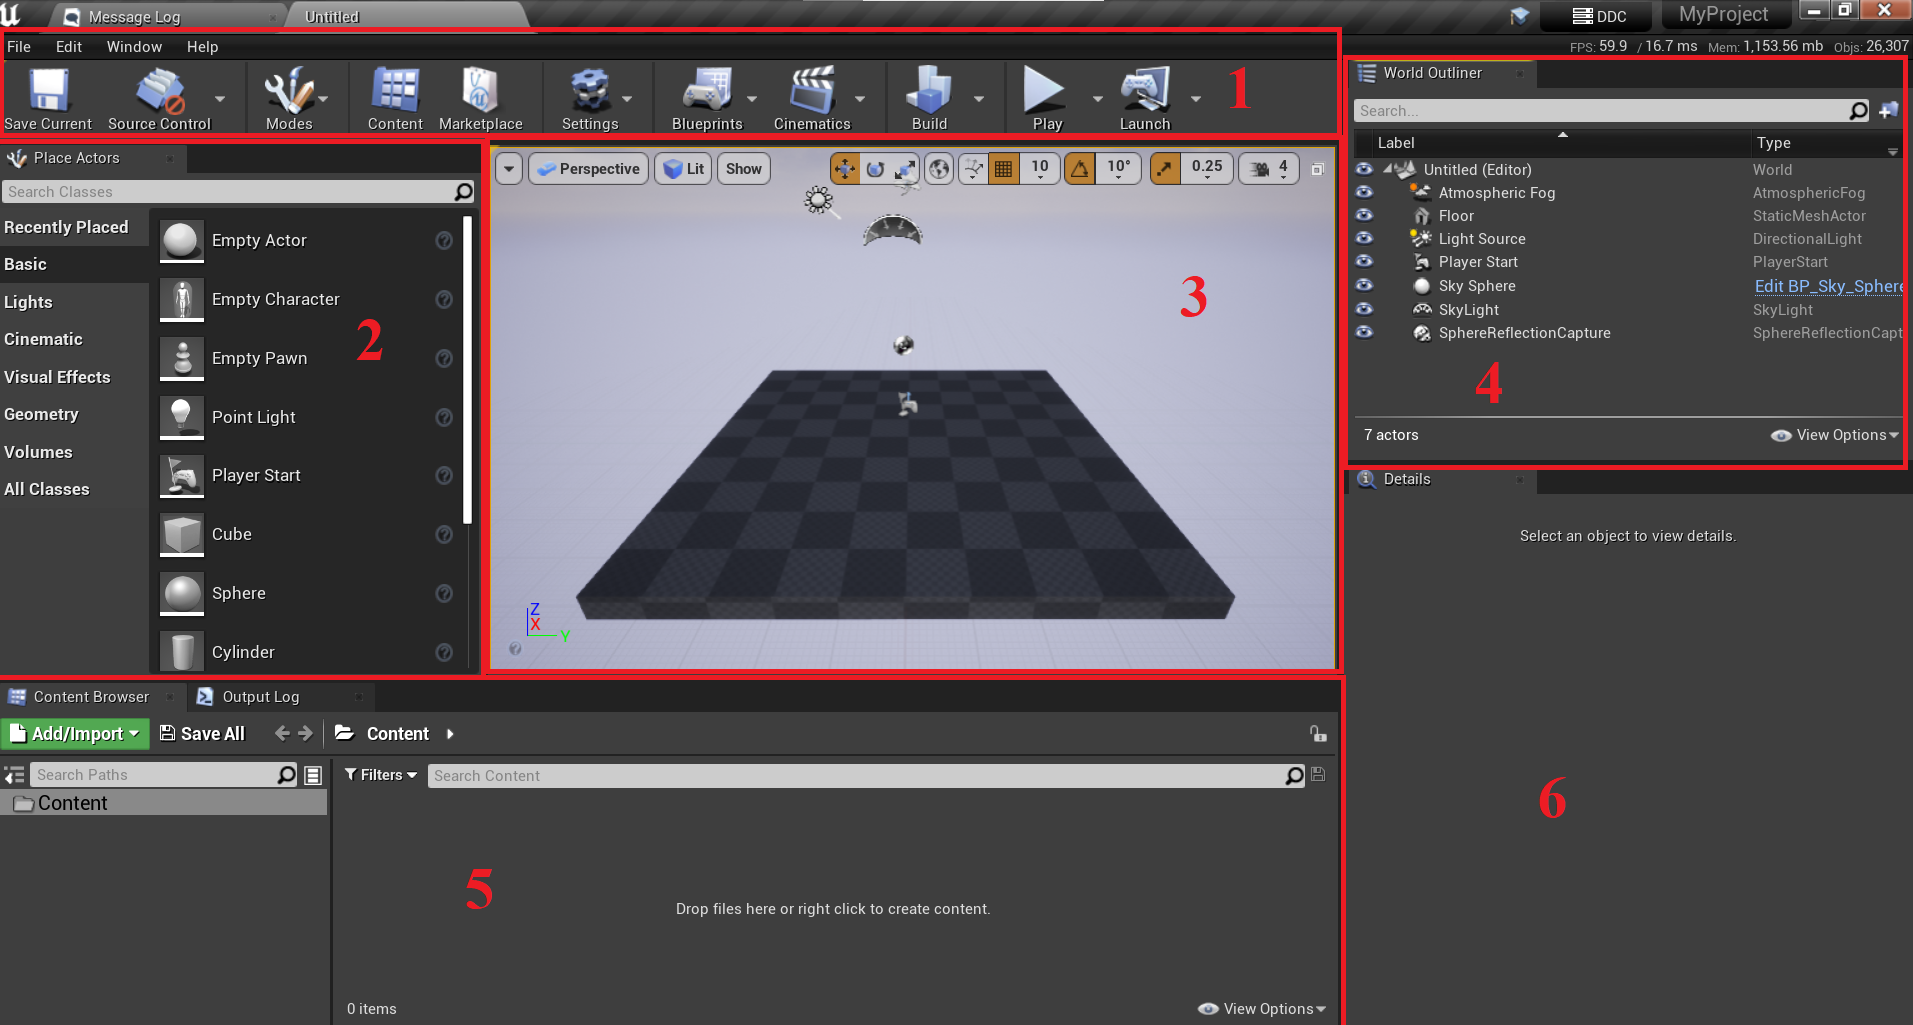
\includegraphics[width=\textwidth,height=\textheight,keepaspectratio]{Figures/Ch2/UnrealEngineEditor.png}}
	\caption{ویرایشگر آنریل}
	\label{fig:Unreal engine Editor}
\end{figure}

\begin{table}[ht]
	\caption{مدلهای تبدیل.}
	\label{tab:MotionModels}
	\centering
	\onehalfspacing
	\resizebox{\textwidth}{!}{
	\begin{tabular}{|r|c|l|r|}
		\hline شماره & نام &  \makecell{توضیح} \\ 
		\hline 1 & نوار ابزار & \makecell{شامل توابع مختلفی است که به صورت معمول استفاده می‌شود}\\ 
		\hline 2 & بازیگران &   \makecell{می‌توان از این قسمت، بازیگر مناسب خود را انتخاب کرده و در صحنه‌ی بازی قرار داد}\\ 
		\hline 3 & درگاه دید
		\LTRfootnote{Viewport} & \makecell{از طریق این پنل می‌توان اشیاء را در محیط قرار داد و بر روی اشیاء قرار گرفته شده کلیک کرد.}  \\ 
		\hline 4 & طرح کلی جهان
		\LTRfootnote{World Outliner} &  \makecell{تمامی اشیاء در مرحله فعلی را نشان می‌دهد. \\
		 می‌توان اشیا را با قرار دادن آن‌ها در پوشا‌ها سازماندهی کرد. همچنین قابلیت جستجو بر اساس نوع را نیز دارد.}\\
		\hline 5 & مرورگر محتوا & \makecell{این پنل تمامی فایل‌های پروژه را نمایش می‌دهد. \\ همچنین می‌توان با ایجاد پوشه فایل‌ها را دسته بندی و مرتب کرد. \\ علاوه بر این با استفاده از نوار جستجو می‌توان فایل موردنظر خود را پیدا کرد}\\ 
		\hline 6 & جزئیات & \makecell{ این پنل برای نمایش یا تغییر ویژگی‌های شئ انتخاب شده است.\\
		 با تغییر ویژگی‌ها تنها ویژگی شی انتخاب شده تغییر پیدا می‌کند.} \\ 
		\hline 
	\end{tabular} }
\end{table}

\section{زبان برنامه‌نویسی}

موتور بازی‌سازی آنریل از زبان برنامه نویسی 
\lr{C++}
به همراه اسکریپ بصری به نام 
\lr{Blueprint}
استفاده می‌کند.

\lr{Blueprint}
یک سیستم برنامه‌نویسی کامل گیمپلی مبتنی بر مفهوم استفاده از رابط‌های مبتنی بر گره برای ایجاد عناصر گیمپلی از درون ویرایشگر است.
این سیستم بسیار منعطف و قدرتمند است زیرا این توانایی را در اختیار طراحان قرار می دهد تا از طیف گسترده ای از مفاهیم و ابزارها که عموماً فقط در دسترس برنامه نویسان هستند استفاده کنند.
\cite{UnrealEngineBlueprint}

\section{رایج‌ترین اصطلاحات}

در این بخش رایج‌ترین اصطلاحات مورد استفاده در هنگام کار با موتور بازی‌سازی آنریل را بررسی می‌کنیم.

\subsection{ پروژه }

یک پروژه آنریل، شامل تمامی محتوای بازی است. 
محتوا می تواند خود به چندین پوشه که بر روی دیسک قرار دارند، تقسیم شود.
بدیهی است که می توان این پوشه‌ها را به صورت دلخواه نامگذاری و سازماندهی کرد.
پنل مروگر محتوا داخل ویرایشگر آنریل همان ساختار راهنمای موجود در پوشه 
\lr{Project}
که بر روی دیسک قرار دارد را نشان می‌دهد.

هر پروژه دارای یک پرونده‌‌ی
\lr{.uproject}
متناظر به خود است.این فایل نحوه ایجاد، باز کردن یا ذخیره یک پروژه است. بنابراین می‌توان چندین پروژه مختلف ایجاد کرد و به صورت موازی بر روی آن‌ها کار کرد.

\subsection{
شئ
}

اشیاء پایه‌ای ترین کلاس موجود در آنریل هستند. آنها مانند بلوک‌های سازنده عمل می‌کنند و دارای بسیاری از عملکرد‌ها و توابع موردنیاز برای دارایی‌ها
\lr{Assets}
هستند.


\subsection{
بازیگران \protect\LTRfootnote{Actors}
}

هر شئ‌ای را که بتوان بر روی صحنه قرار داد مانند دوربین، مش استاتیک، محل شروع بازی و ... را بازیگر
\LTRfootnote{Actor}
می‌گویند.
بازیگران از تبدیل‌های سه‌بعدی مانند انتقال، دوران و تغییر مقیاس پشتیبانی می‌کنند.
آن‌ها را می‌توان از طریق کد‌های گیمپلی (
	\lr{C++}
	یا برنامه‌کار 
	\LTRfootnote{Blueprint}
)
ایجاد کرد و یا از بین برد.

\subsection{تغییر نوع داده 
\protect\LTRfootnote{Casting}}

تغییر نوع داده، عملی است که طی آن بازیگری از یک کلاس را گرفته و سعی می‌کند به گونه‌ای رفتار کند که گویی از کلاس دیگری است.
این عمل ممکن است موفقیت آمیز باشد و یا شکست بخورد. در صورت موفقیت آمیز بودن می‌توان به توابع کلاسی که به آن تغییر داده شده دستیابی پیدا کرد.

